Considering the limitations outlined in section
\ref{sssec:mapreduce_limitations}, Vinod Kumar Vavilapalli et
al. presented YARN \cite{Vavilapalli:2013:AHY:2523616.2523633} the new
resource management layer that was adopted in Hadoop 2.0. The new
Hadoop stack now is depicted in Figure \ref{fig:yarn_hadoop1_hadoop2_arch} where YARN is the
cluster resource management module and MapReduce is one out of plenty
applications running on top of YARN. This architectural transformation
paved the way for a wide variety of frameworks like
Apache Spark \cite{apache_spark}, Apache Flink \cite{apache_flink},
Apache Pig \cite{apache_pig}, etc to run on the
Hadoop platform like any other YARN application.

\begin{figure}
\centering
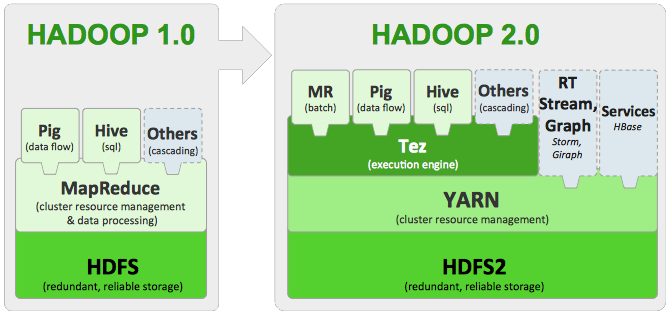
\includegraphics[scale=0.6]{resources/images/Background/hadoop1_hadoop2_arch.png}
\label{fig:yarn_hadoop1_hadoop2_arch}
\caption{Hadoop 2.0 stack \cite{hortonworks_hadoop_stack}}
\end{figure}

The new architecture of Hadoop 2.x separates the resource management
functions from the programming model. It delegates the
intra-application communication and the tracking of the execution flow
to per-job components. That unlocks great performance improvements,
improves scalability and enables a wide variery of frameworks to share
the cluster resources in a very gentle way.

YARN uses three main components to provide a scalable and fault
tolerant resource management platform. The first component is the
\emph{ResourceManager} (RM), a per-cluster daemon that tracks resource
usage and node liveness and schedules jobs on the cluster. The second
component is a per-node \emph{NodeManager} (NM) which is responsible
for monitoring resource availability on the specific node, reporting
faults to RM and managing container lifecycle. Finally, there is the
\emph{ApplicationMaster} (AM) which coordinates the logical plan of a
single job, manages the physical resources offered by the RM and
tracks the execution of the job.

\subsubsection{ResourceManager}
\label{sssec:rm}
ResourceManager stuff...

\subsubsection{ApplicationMaster}
\label{sssec:am}
ApplicationMaster stuff...

\subsubsection{NodeManager}
\label{sssec:nm}
NodeManager stuff...

\subsubsection{YARN HA \& fault tolerance}
\label{sssec:yarn_ha}
YARN HA and fault tolerance stuff...
